% 
%jff-notes
%
\documentclass[10pt]{article}
\usepackage[pdftex]{graphicx}
\usepackage{amssymb}
\usepackage{latexsym}
%\usepackage{relsize}
\usepackage{textcomp}
%processed for 10 pt 
%\documentstyle[epsf,psfig]{article}
%\documentstyle[epsf]{article}
\oddsidemargin 0pt
\topmargin -0.0cm
\textwidth 6.2in
\textheight 8.5in
\baselineskip 18pt
%\renewcommand{\baselinestretch} {1.5}
\newenvironment{nitemize}
   {\begin{list}{\begin{math}\bullet\end{math}}%
      {\setlength{\leftmargin}{5mm}
       \setlength{\topsep}{1mm}
       \setlength{\parsep}{0in}
       \setlength{\itemsep}{.7mm}}}%
   {\end{list}}

\newcommand{\fract}[2]{\frac{\textstyle #1}{\textstyle #2}}
\newcommand{\trans}[3]{#1 \stackrel{#2}{\longrightarrow} #3}
\newcommand{\notrans}[3]{#1 \stackrel{#2}{\not\! \longrightarrow} #3}
\bibliographystyle{plain}
\begin{document}
\title{An SDRuno plugin for DRM30\\
{small user's guide {\footnote {\copyright J van Katwijk}}\\
Revised edition of the plugin}}
\author{
Jan van Katwijk\\
Lazy Chair Computing \\
The Netherlands\\
{\em J.vanKatwijk@gmail.com}}
%\date{}
\maketitle
%\baselineskip 22pt
\ \\
\ \\
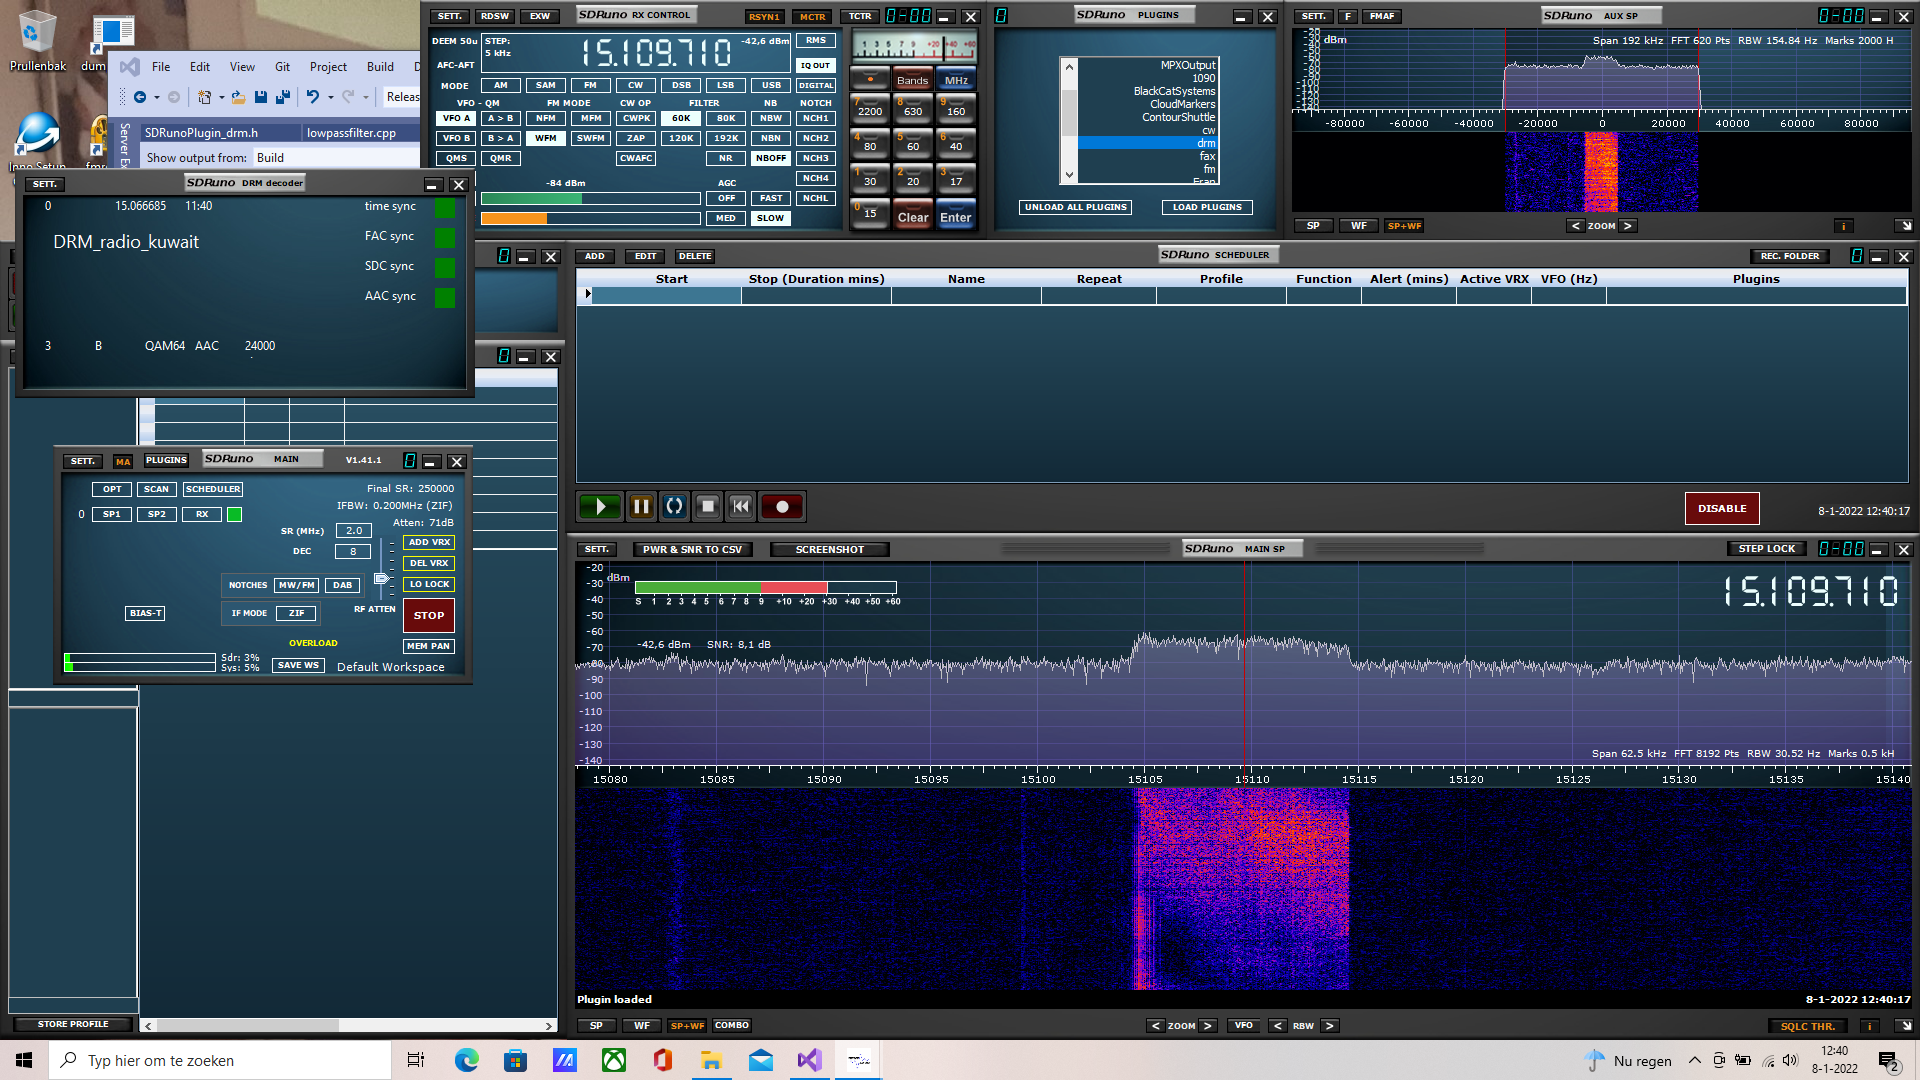
\includegraphics[width=160mm]{drm-decoder.png}
\ \\
\section{Introduction}
DRM, Digital Radio Mondiale, is a system for digital radio on medium and
short waves up to 30 MHz. This form of DRM is sometimes called DRM30, a variant
of DRM, called DRM+, is meant to operate in the FM band,
\par 
DRM is not very popular in western Europe, I receive during daytimes the
transmission from Radio Kuwait, and in the evening transmissions from
Radio Romenia International.
In the past there were transmissions from e.g. Spain, Nigeria and India,
Spain stopped the DRM transmissions around 2015, and
I do not hear Nigeria nor India anymore.
I have to admit though that my antenna equipment is rather limited,
for shortwave I use an in-house loop antenna with a simple amplifier.
\par
The front page shows the reception of a transmission of Radio Romenia at 7350 KHz, Radio Romenia transmits daily in different languages.
\par
This document describes a {\em plugin} for decoding DRM30,
a plugin developed for the SDRuno environment.
\section{Installing}
As  the other plugins for SDRuno, the plugin is implemented as
a dll, i.e. a {\em dynamic load library}, and it should be installed
in the folder for community plugins.
\par
The recent standard for DRM supports, next to AAC encoded audio, xHE-AAC 
encoded audio. The {\em libfdk-aac-2} decoder is capable of handling both.
The plugin uses this decoder for AAC and xHE-AAC decoding (note that so far
I did not receive any DRM transmission with service(s) encoded as xHE-AAC).
\begin{itemize}
\item
{\em libfdk-aac-2.dll}, for the decoding of the AAC and xHE-AAC data is the main one.
However, running this dll requires two additional dll's to be installed
\item {\em libgcc\_s\_dw-1.dll}, and
\item {\em libwinpthread-1.dll}
\end{itemize}
As said, these libraries are needed for convertings the AAC
(or xHE-AAC) blocks to PCM samples, the last step in the
plugin. The PCM samples are sent to the SDRuno system for the
actual sound output.
\par
{\em If (one of) these libraries is NOT installed, the plugin will work
with limited functionality: no sound will be decoded}.
In that case the plugin will
show a message to invite you to install the library (libraries)

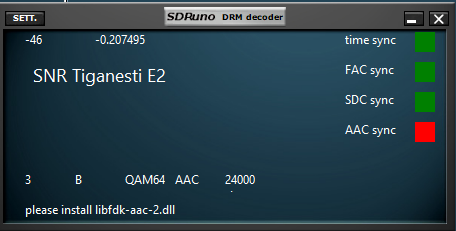
\includegraphics[width=100mm]{lib-not-found.png}

Copies of the libraries can be found in the "the-dll" folder
in the repository.
Being a Linux developer, I do not understand much of Windows, but I
installed these libraries in the folder
where the Uno stuff is stored:
\begin{verbatim}
C:\\Program Files(x86)\\SDRuno
\end{verbatim}
\section{Running the plugin}
The DRM signal (in the common modes)
has a spectrum with a width of 10 KHz. SDRuno usually shows
a much wider spectrum. On a 2 MHz wide spectrum 10 KHz takes 1/200-th part
and is therefore not (hardly) visible. Furthermore, while the plugin
is ablwe to correct for frequency offsets, tuning should be as precise
as possible, preferably with an offset less than 3 or 400 Hz.
\par
The plugin operates using the {\em IQOUT} option of SDRuno. Selecting
this option - the plugin itself will do so - gives an input rate
of 192000 complex samples per second. The plugin software will take
care of filtering out a band of 10 Khz and decimating to 12000 samples/second.
\par
To get a decent view on the signal, most likely needed to fine-tune,
it is advised to select {\em on the main widget samplerate 2000000,
and a suitable decimation factor} (I use a decimation factor 8, leading to a
spectrum with a width of 250 KHz).
Using the {\em zoom}  option, the spectrum in the picture at the
top of this paper takes just over 60 Khz,
The SDRuno filter is set to 60 KHz.

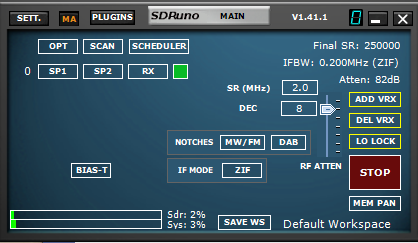
\includegraphics[width=100mm]{drm-main-widget.png}

The spectrum of the DRM signal clearly shows: other than FM or AM signals 
no visible carrier or peak (the signal consist of over 200 carriers
with a mutual distance of just over 45 Hz).

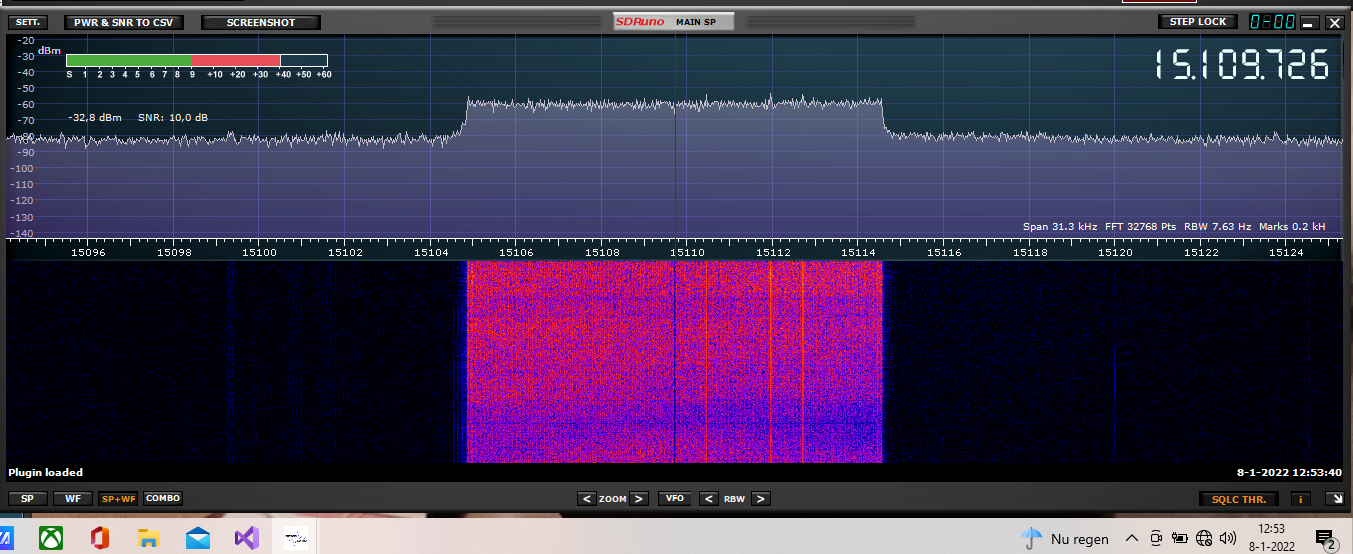
\includegraphics[width=150mm]{drm-zoom.png}

Note that in order to be able to decode the signal, the signal should
have a reasonable signal strength.  The figure here indicates that the signal strength is about 10dB.
\par
What the waterfall shows is - apart from a nice color spectrum - three
lines, coloured slightly brighter red. These lines correspond with special elements
in the spectrum that will help the receiver to synchronize with
the incoming signal.

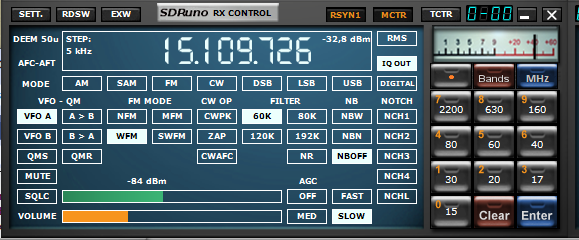
\includegraphics[width=100mm]{drm-receiver-widget.png}

\section{The widget}
On selecting the plugin, the software starts reading in samples,
trying to reach synchronization, etc.
The detected {\em mode} (one of Modes {\em A, B, C})  and the {\em spectrum}
(one of 1 .. 3) are displayed, as is the way the bits of the
audio content are encoded (usually QAM16 or QAM64), followed by
the decoding of the audio (either AAC or xHE-AAC) and the output
sample rate.
\par

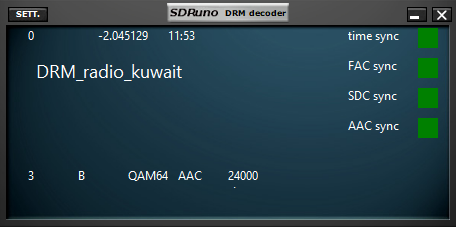
\includegraphics[width=100mm]{drm-decoder-widget-1.png}

At the top left, one sees two numbers, telling the offset of the selected
frequency. The first number indicates the so-called {\em coarse} offset,
which is (should be) reasonably stable, the second one tells the
so-called {\em fine} offset, which ranges between -30 .. 30 and is
- in most cases - continuously changing.

Note that the {\em coarse offset} for radio Kuwait is here 0, but the
tuner was set app 280 Hz lower than the offical transmitter frequency
of 15110 KHz. The {\em fine offset} is just -2 Hz.

The number to the right, 11.53, tells the 
time of the transmission (in UTC), not all transmissions show the
transmission time.
\par
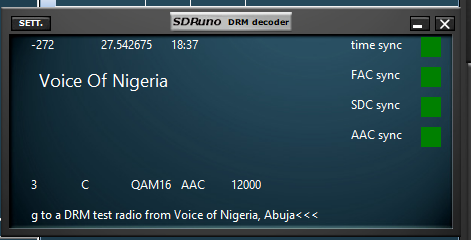
\includegraphics[width=100mm]{drm-decoder-widget.png}
\par
The second picture, taken from a recording from a few years back,
shows that the transmission was in mode C, the audio was encoded as QAM16
rather than QAM64, and the audio output samplerate was 12000.
Note that the bottom line of the widget can be filled with a message
as was done by the Voice of Nigeria.
\par
Processing the input takes 4 steps
\begin{itemize}
\item trying to reach time synchronization;
\item then, trying to decode the FAC (Fast Access Channel) that contains
some general information on the transmission;
\item trying to decode the SDC (Service Description Channel), that contains
detailed information on the service(s) and their decoding;
\item trying to decode the AAC frames of the selected service.
\end{itemize}
The state of each of these "processes" is shown at the right side,
from top to bottom an indicator for {\em time synchronization}, success
in {\em FAC} decoding, success in {\em SDC} decoding and, finally, success
with {\em AAC} decoding. 
If all these indicators are {\em green}, there will be sound, if one or
mode of the indicators are red, some process parts fail with the given input
and no sound can be emitted.
\paragraph{Services}

Most DRM transmissions carry a single service (as shown by the pictures
above).
The DRM technique, however, allows carrying more than one service (actually, up to 4). If a single service is carried, that service is - by default -
the selected one and its content is decoded automatically.
If, however, the transmission carries two services, both service
names are shown and - by default -  the first one is selected.
\par
Clicking with the mouse on any of the two services will select that service,
and to avoid ambiguity, the widget indicates which service is the selected one.

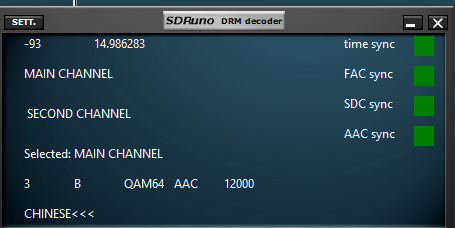
\includegraphics[width=100mm]{drm-two-services.png}

\section {Notes on the implementation}
The implementation of this plugin is almost a twin sister of the
{\em drm-receiver} implementation for Linux, this twin
implementation is a rewrite of my DRM backend for the sw software,
the latter is slightly more extended since it supports - although untested -
data transmissions.
\par
This DRM plugin has some limitations, when compared to the standard:
\begin{itemize}
\item the plugin does not provide support for data transmissions, other than
texts appearing as program associated data;
\item the plugin supports up to two audio services;
\item the plugin - in its current form - does not support spectra larger
than 10 KHz;
\item the plugin does not support DRM+.
\end{itemize}
\end{document}


